% UPAR 2027 Track 2 paper. WACV 2026 author kit, the format required by the RWS workshop at WACV 2027.
% English submission copy of main_vi.tex. Writing rules: skill upar-paper-rules; terminology: PLAN.md.
% Numbers: analysis/*.json and analysis/knn_logs_2026-10-11.txt. Figures: analysis/make_figs.py --lang en --q 2876.
\documentclass[10pt,twocolumn,letterpaper]{article}

%%%%%%%%% PAPER TYPE: anonymous review version (the kit requires a track option in review mode)
\usepackage[review,algorithms]{wacv}
%\usepackage{wacv}  % camera-ready version

%
% --- inline annotations
%
\newcommand{\red}[1]{{\color{red}#1}}
\newcommand{\todo}[1]{{\color{red}#1}}
\newcommand{\TODO}[1]{\textbf{\color{red}[TODO: #1]}}
% --- disable by uncommenting  
% \renewcommand{\TODO}[1]{}
% \renewcommand{\todo}[1]{#1}


\usepackage{booktabs}
\usepackage{amsmath}
\usepackage{graphicx}
\graphicspath{{figs/}}

\definecolor{wacvblue}{rgb}{0.21,0.49,0.74}
\usepackage[pagebackref,breaklinks,colorlinks,allcolors=wacvblue]{hyperref}
\usepackage[capitalize]{cleveref}

\def\wacvPaperID{*****}
\def\confName{WACV}
\def\confYear{2027}

\title{Rank by Likelihood, Smooth over Neighbors: Foundation Encoders\\for Attribute-Based Person Retrieval on Unseen Cameras}
\author{Anonymous WACV Algorithms Track submission}

\begin{document}
\maketitle

%=====================================================================
\begin{abstract}
In this paper, we present our solution to Track~2, attribute-based person retrieval, of the UPAR Challenge 2027 at the WACV 2027 Real-World Surveillance workshop. Attribute-based person retrieval finds a person in surveillance images from a description alone, such as gender, age, clothing colors and accessories, without an example image of that person. The task is hard when the images come from cameras that are not in the training data, because the attribute probabilities predicted by the model shift on new cameras. The usual method ranks images by the L1 distance between the predicted attribute probabilities and the query, and in the two previous editions no team beat the organizers' baseline on this track. We fine-tune two foundation encoders, DINOv3 and CLIP, separately and make three changes. Each image is scored by the log-likelihood of the exact query instead of the L1 distance. The models are also trained with a cross-entropy loss over groups of mutually exclusive attributes, such as age ranges or upper-body colors. The logits of each image are smoothed with those of its nearest neighbors in the gallery, found with DINOv3 features. In leave-one-dataset-out experiments, all three changes raise mADM on both held-out datasets, and the likelihood score alone raises all six retrieval metrics. The smoothing step needs no training, and with features of the pretrained DINOv3 encoder it raises mADM for every model we tested. In contrast, recalibrating the probabilities after training with data from the source datasets lowers mADM. On the hidden challenge test set, our system reaches an mADM of 0.6817.
\end{abstract}

\begin{figure*}[t]
\centering
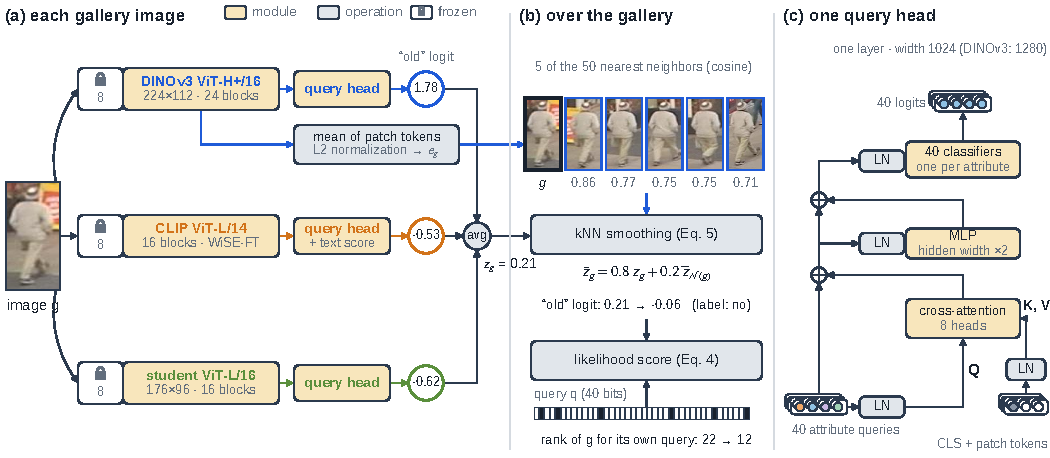
\includegraphics[width=\linewidth]{arch_en.pdf}
\caption{(a) The three models on one image $g$ of the PETA gallery. Each encoder freezes the patch embedding and the first eight blocks (lock) and fine-tunes the other blocks together with a query head. The circles are the logits of the old-age attribute (Age-Old) from the three models of the PETA fold, which saw no PETA image in training, and their mean is $z_g$. In the same forward pass, the L2-normalized mean of the patch tokens of DINOv3 ViT-H+/16 is the appearance feature $e_g$. (b) Five of the 50 nearest neighbors of $g$ by cosine similarity of $e_g$, all the same person in other frames. These neighbors are found with the submitted DINOv3 model, which saw these validation images in training. After kNN smoothing (\cref{eq:knn}), the old-age logit changes sign and agrees with the label. For the query made from the labels of $g$, the rank of $g$ under the likelihood score (\cref{eq:ll}) improves from 22 to 12. (c) One query head. The three models share this design, and the query head of the CLIP model also adds a text score.}
\label{fig:arch}
\end{figure*}

%=====================================================================
\section{Introduction}
\label{sec:intro}

Attribute-based person retrieval finds a person in surveillance images from a verbal description alone, such as gender, age, clothing colors and accessories, without an example image of that person~\cite{upar}. It is usually solved by recognizing the attributes of each image and comparing the predictions with the query~\cite{upar,specker21}. A major difficulty appears when the images come from cameras never seen in training. Resolution, viewpoint and lighting change between cameras, and each training dataset labels attributes by its own rules. Attribute probabilities that fit the training cameras can therefore shift on a new camera, and the ranking built from them shifts too.

The UPAR Challenge 2027 follows the 2023 and 2024 editions~\cite{upar23,upar24}. Models are trained on PA100k~\cite{pa100k}, PETA~\cite{peta} and Market-1501~\cite{market,marketattr} and tested on images from other cameras. In the two previous editions, no team beat the organizers' baseline on the retrieval track, although many teams beat it on the attribute recognition track~\cite{upar23,upar24}. The 2024 report suggests that models become overconfident or underconfident on new cameras, and that these shifted probabilities distort the distance to the query~\cite{upar24}. The sample code of this year's challenge still ranks images by the L1 distance~\cite{starterkit}.

In this paper, we present our solution to Track~2 of the UPAR Challenge 2027. We use two foundation encoders with different pretraining, DINOv3~\cite{dinov3} and CLIP~\cite{clip}. Each is fine-tuned separately with a query head~\cite{q2l}, and their logits are averaged together with those of a student distilled from two teachers~\cite{hinton,patient} (\cref{fig:arch}). Our system makes three changes to how predictions become a ranking. First, each image is scored by the log-likelihood of the exact query instead of the L1 distance, similar to the way DAP scores a class from its attributes~\cite{dap}. Second, this score treats the attributes as independent, while many attribute groups are mutually exclusive, so the models are also trained with a cross-entropy loss over each such group. Third, the logits of each image are mixed with those of its nearest neighbors in the gallery, found with appearance features from the same DINOv3 forward pass. This step is similar to database-side augmentation in image retrieval~\cite{turcot,gordo}, and the Track~2 rules allow such automatic re-ranking as long as it uses no private information about the hidden test set~\cite{rules}.

To evaluate how effective each change is, we test every choice on a dataset that is not in the training data and with the same trained models, so that differences come only from the step under test. We also check the two findings on scoring and on recalibration with the models of our development phase, and we test the full system on the hidden test set. The main contributions of this paper are below.
\begin{itemize}
\item Scoring by the log-likelihood of the exact query beats the L1 distance on every retrieval metric, on both held-out datasets and for every development model. The L1 distance ranks an image that is confidently wrong on a single attribute above an exact match that is slightly uncertain on many attributes.
\item Miscalibration is real but cannot be fixed after training. Recalibration fitted on the labels of the held-out dataset raises mADM, but recalibration fitted on the source datasets lowers it. The source data show a similar amount of miscalibration as the held-out dataset, but the direction of the error for each attribute differs between the two.
\item A cross-entropy loss over groups of mutually exclusive attributes raises mADM on both held-out datasets, both alone and together with kNN smoothing.
\item kNN smoothing needs no training and does not depend on the attribute model. With features of the pretrained DINOv3 encoder, it raises mADM for every development model on both held-out datasets, and the gain comes from the appearance features, not from averaging in general.
\end{itemize}

%=====================================================================
\section{Related work}
\label{sec:related}

\paragraph{Attribute-based person retrieval.} Methods for attribute-based person retrieval either recognize attributes and compare the predictions with the query, or learn a shared space for attribute descriptions and images~\cite{upar}. The first approach gives results that are easy to explain, because each part of the score belongs to one attribute~\cite{upar}. For this approach, combining the scores of many attribute classifiers has been studied before. Siddiquie \etal rank images for multi-attribute queries and model the correlations between attributes~\cite{siddiquie}. Scheirer \etal turn the raw score of each classifier into a probability before combining the scores, and this normalization needs no labels~\cite{scheirer}. DAP scores a class by the product of the attribute probabilities of that class, divided by their prior probabilities~\cite{dap}. Our likelihood score has the same product form but does not divide by the priors. For UPAR, Specker and Beyerer show that methods at that time used the Euclidean distance between the query and the prediction. They propose a distance that takes the output distribution of the classifier into account, together with recalibration and a weight for each attribute based on its prediction error~\cite{specker21}. They later propose a model that works well both for single attributes and for retrieval, together with the mADM metric~\cite{specker23}. The challenge baseline is a ConvNeXt with one fully connected layer, trained with a weighted cross-entropy loss~\cite{upar23}. Among these works, \cite{specker21} is directly related to ours, because it also replaces the distance and recalibrates the probabilities. We use the probability of an exact match instead of a distance, and we measure directly whether recalibration learned on source data still holds on a dataset that is not in the training data.

\paragraph{Calibration under distribution shift.} Recalibration maps the scores of a classifier to probabilities with a small function fitted on labeled data. Platt scaling fits a sigmoid to the scores~\cite{platt}. Temperature scaling uses one factor for all classes and removes most of the miscalibration of neural networks on data from the same distribution~\cite{guo}. Both need labeled data from the same distribution as the test data. Ovadia \etal show that the calibration of deep models gets worse under distribution shift, even after temperature scaling~\cite{ovadia}. Kull and Flach split a proper scoring rule into several terms, and the calibration term is the part that an optimal recalibration map can remove~\cite{kull}. We use this term to compare the miscalibration of the same model on source data and on the held-out dataset.

\paragraph{Using the gallery for ranking.} Besides correcting each prediction on its own, a ranking can also use the other images of the gallery. In person re-identification, k-reciprocal re-ranking uses the neighbor relations between the query and the gallery images to re-rank the gallery~\cite{kreciprocal}. In image retrieval, query expansion builds a new query from the top results~\cite{chum07}. Database-side augmentation replaces the representation of each database image by a combination of the image and its neighbors~\cite{turcot,arandjelovic,gordo}. These methods compare the query and the gallery in the same feature space. In attribute-based retrieval, however, the query is a binary vector and has no image. We therefore apply the idea of database-side augmentation to the attribute logits of the gallery, while the neighbors are found in the image feature space. LAME~\cite{lame} also adjusts the outputs of a model with a neighbor graph of the test samples. LAME solves an optimization problem for classification, while our kNN smoothing is a single weighted average with fixed weights.

\paragraph{Foundation encoders and ensembles.} The logits that kNN smoothing averages come from two fine-tuned foundation encoders, DINOv3~\cite{dinov3} and CLIP~\cite{clip}, which are pretrained in different ways. Fine-tuning can distort pretrained features and lower accuracy when the data distribution changes~\cite{lpft}. WiSE-FT reduces this effect by interpolating between the pretrained and the fine-tuned weights~\cite{wiseft}. Averaging the predictions of several models, each trained on its own, gives more accurate predictions and more reliable probabilities than each model alone~\cite{deepens}. Distillation transfers the predictions of teachers to a student~\cite{hinton}, and it works better when the teacher and the student see the same augmented image and training is long enough~\cite{patient}. We use these known parts to obtain good attribute probabilities, and we focus on the step that turns the probabilities into a ranking.

%=====================================================================
\section{Method}
\label{sec:method}

Our system takes a query of 40 binary attributes and a gallery of cropped person images, and returns a ranking of the whole gallery (\cref{fig:arch}). Three attribute recognition models run on each image, and the mean of their logits is smoothed with the logits of similar images in the gallery. Each image is then scored by the log-likelihood of the query, and the gallery is ranked by this score.

\paragraph{Task and metric.} The gallery is a set of cropped person images. Each query is a vector $q\in\{0,1\}^{K}$ with $K=40$ attributes. The challenge creates one query for each distinct label vector in the gallery, and an image is an exact match for a query when all 40 of its labels equal the query. For each query, the system returns a ranking of the whole gallery. The main metric is mADM~\cite{specker23}. Let $\mathrm{dom}(q,g)$ be the share of attributes on which image $g$ agrees with $q$. This agreement is normalized per query,
\begin{equation}
\mathrm{ndom}(q,g)=\max\Big(0,\frac{\mathrm{dom}(q,g)-\overline{\mathrm{dom}}_q}{\max_{g'}\mathrm{dom}(q,g')-\overline{\mathrm{dom}}_q}\Big),
\label{eq:ndom}
\end{equation}
where $\overline{\mathrm{dom}}_q$ is its mean over the gallery. Let $r_1<\dots<r_R$ be the ranks of the $R$ exact matches and $g_{(j)}$ the image at rank $j$. Then
\begin{equation}
\mathrm{ADM}(q)=\frac1R\sum_{m=1}^{R}\frac{1}{r_m}\sum_{j\le r_m}\mathrm{ndom}\big(q,g_{(j)}\big),
\label{eq:adm}
\end{equation}
and mADM is the mean of ADM over all queries. ADM is like average precision, but each image ranked before an exact match counts with its agreement instead of 0 or 1. The exact matches therefore decide where the score is taken, and near matches ranked before them still earn part of the score. We also report mAP, mINP, Rank-1, Rank-5 and Rank-10, as on the leaderboard. All metrics are multiplied by 100 and given in points.

\paragraph{Three attribute recognition models.} The DINOv3 model uses the DINOv3 ViT-H+/16 encoder~\cite{dinov3} with 840M parameters. The CLIP model uses the OpenAI CLIP ViT-L/14 image encoder~\cite{clip} with 303M parameters. Both read $224\times112$ images. Each encoder has a one-layer query head~\cite{q2l,mldecoder} (\cref{fig:arch}c). Forty learned attribute queries read the image tokens through cross-attention, and then an MLP with a residual connection and one classifier per attribute turn each query into one logit. The query head of the CLIP model adds a text score to each logit. This score compares the CLS token, after the pretrained CLIP projection, with a text direction for each attribute. The text direction is the text embedding of a sentence that describes the attribute minus the text embedding of the neutral sentence \texttt{a person}. After fine-tuning, the encoder weights of the CLIP model are interpolated with WiSE-FT~\cite{wiseft}, with a weight of 0.7 for the fine-tuned weights and 0.3 for the pretrained weights. The third model is a DINOv3 ViT-L/16 student that reads $176\times96$ images. The student learns from the labels and from the mean logits of two teachers, DINOv3 ViT-L and CLIP ViT-L, with a weight of 0.8 on the distillation loss~\cite{hinton}. Half of the student's batches are mixed with mixup or CutMix and learn only from the outputs of the teachers on the mixed images, following function matching~\cite{patient}.

The three models are trained with binary cross-entropy, label smoothing of 0.05~\cite{szegedy} and DeepMAR weights for each attribute~\cite{deepmar}. The patch embedding and the first eight blocks of each encoder are frozen. The other blocks are fine-tuned with AdamW, with a learning rate of $5\cdot10^{-5}$ for the top block that decays by a factor of 0.75 per block below, and a ten times higher learning rate for the query head. All models use a batch size of 64 and an exponential moving average (EMA) of the weights. The DINOv3 and CLIP models are trained for three epochs, and the student for 20 epochs. Many attributes form mutually exclusive groups, namely three age ranges, three hair lengths, two lower-body clothing types, 12 upper-body colors and 12 lower-body colors. With 40 independent sigmoids, the model can put probability on label vectors that never occur, such as two age ranges at once. We therefore also train the DINOv3 and CLIP models with a cross-entropy loss over each such group (group CE),
\begin{equation}
L_{\mathrm{gce}}=\sum_{G}\mathrm{CE}\big(\mathrm{softmax}(z_G),\,y_G\big),
\label{eq:gce}
\end{equation}
where $z_G$ are the logits of the attributes in group $G$ and $y_G$ is the single positive attribute of the group. This term is computed only on images in which the group is fully labeled and has exactly one positive label, and it is added to the main loss with a weight of 0.5. The submitted models are trained on the training and validation splits of all three datasets. The logits of the three models are averaged into $z_g\in\mathbb{R}^{40}$ for each image $g$, and $p_g=\sigma(z_g)$. No offset or per-attribute threshold is added after training.

\paragraph{Likelihood score.} The L1 distance $d(q,g)=\sum_k|q_k-p_{gk}|$ equals the expected number of attributes on which image $g$ is wrong. It therefore cannot tell one certain error from many small doubts. An image that matches 39 attributes almost surely and is wrong on one attribute with $p=0.04$ has a distance of about 1. An exact match that is only 95\% sure of each attribute has a distance of 2, so it is ranked after the first image. Yet the first image can hardly be an exact match, while the second very likely is. ADM takes its score at the positions of the exact matches, so a better score is the probability that the image is an exact match for the query. The probability ranking principle states that ranking by the probability of relevance is optimal when these probabilities are accurate~\cite{prp}. If the attributes are independent given an image, the log-probability of an exact match is
\begin{equation}
\begin{aligned}
s(q,g)&=\sum_{k}\big[q_k\log p_{gk}+(1-q_k)\log(1-p_{gk})\big]\\
&=q^\top\log\frac{p_g}{1-p_g}+\sum_k\log(1-p_{gk}).
\end{aligned}
\label{eq:ll}
\end{equation}
The second form shows that the scores of all query--image pairs are a matrix product plus one term for each image. Images with a larger $s$ are ranked first. For the two images above, the exact match has $s=40\log0.95\approx-2.1$, while the image that is wrong on one attribute has $s\approx\log0.04\approx-3.2$. Probabilities are clipped to $[10^{-4},1-10^{-4}]$, so that a single attribute cannot push the score to minus infinity.

\paragraph{kNN smoothing.} The images of a surveillance gallery are not independent, because the same person often appears in several frames or cameras. If we can find images with the same label vector as a given image, averaging their predictions reduces the noise in the prediction for that image. These images must be found without labels and without the query. The appearance feature $e_g$ of image $g$ is the mean of the last-layer patch tokens of the DINOv3 encoder, L2-normalized, and it is computed in the same forward pass that predicts the attributes. Let $\mathcal{N}(g)$ be the $k$ nearest neighbors of $g$ among the other gallery images, by cosine similarity of the appearance features. The smoothed logits are
\begin{equation}
\tilde z_g=(1-\alpha)\,z_g+\frac{\alpha}{k}\sum_{n\in\mathcal{N}(g)}z_n,
\label{eq:knn}
\end{equation}
and $\sigma(\tilde z_g)$ replaces $p_g$ in \cref{eq:ll}. The factor $\alpha$ keeps most of the weight on the image's own prediction, so a wrong neighbor cannot replace that prediction. We use $k=50$ and $\alpha=0.2$. For the PETA gallery, this step takes 0.1 seconds on a GPU. It is applied in the same way to every gallery with fixed $k$ and $\alpha$, and it uses no labels, file paths or folder structure of the test set. The Track~2 rules allow automatic post-processing, refinement and re-ranking, as long as they do not exploit or use any private information about the hidden test set~\cite{rules}.

%=====================================================================
\section{Experiments}
\label{sec:exp}

The submitted system combines the likelihood score, group CE and kNN smoothing. The following subsections measure the contribution of each change, test recalibration after training and the role of the two encoders, and then check the system on the hidden test set.

\subsection{Evaluation protocol}
\label{sec:protocol}
We use a leave-one-dataset-out protocol. Each fold holds out one dataset completely, and its models see none of its images in training. The models are trained on the training splits of the other two datasets, the source datasets. They are tested on the validation split of the held-out dataset. This split is the gallery, and each distinct label vector in it is a query. In the PETA fold, PETA is held out, and the gallery has 6,963 images and 1,763 queries. In the Market-1501 fold, the gallery has 16,458 images and 956 queries. We do not use the fold that holds out PA100k, because its training set has only 18.7k images. The fold models are trained as described in the method, each on one RTX 5090 GPU. The DINOv3 model is trained with one seed. The CLIP model is trained with two seeds, and each metric of a model or an ensemble that includes CLIP is the mean over the two seeds. No parameter is chosen on the hidden test set.

To check the two findings on scoring and on recalibration with more models, we also use 49 models from our development phase whose logits on the held-out dataset were saved. These development models include ViT and ConvNeXt encoders of several families at sizes B, L and H. They split into 42 models of the PETA fold, 5 models of the Market-1501 fold and 2 models of the PA100k fold.

\subsection{How should each image be scored?}
\label{sec:score}

\begin{table}[t]
\centering
\small
\setlength{\tabcolsep}{3.2pt}
\begin{tabular}{@{}llcccccc@{}}
\toprule
Fold & Score & mADM & mAP & mINP & R-1 & R-5 & R-10 \\
\midrule
PETA & L1 & 62.88 & 24.03 & 18.67 & 21.75 & 39.59 & 47.22 \\
 & likelihood & \textbf{69.91} & \textbf{35.51} & \textbf{29.08} & \textbf{31.57} & \textbf{54.68} & \textbf{63.07} \\
\midrule
Market & L1 & 69.29 & 25.08 & 8.97 & 32.53 & 51.46 & 58.00 \\
 & likelihood & \textbf{74.90} & \textbf{34.39} & \textbf{16.84} & \textbf{37.97} & \textbf{61.30} & \textbf{70.87} \\
\bottomrule
\end{tabular}
\caption{The L1 distance and the likelihood score (\cref{eq:ll}) on the same probabilities of the DINOv3 + CLIP ensemble (CLIP with text score and WiSE-FT). The likelihood score is higher on all six metrics on both held-out datasets. All numbers are in points.}
\label{tab:score}
\end{table}

\begin{figure}[t]
\centering
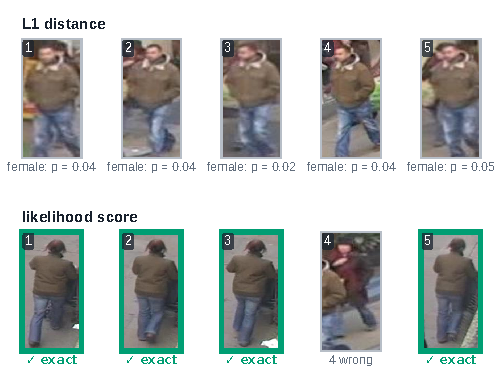
\includegraphics[width=\linewidth]{l1ll_en.pdf}
\caption{Top five images for one query on the PETA gallery, with the DINOv3 + CLIP ensemble of the PETA fold. The query describes an adult woman with short hair, a brown top and blue trousers or shorts. In the top row, ranked by the L1 distance, all five images show one man who differs from the query only in the female attribute (Gender-Female), and the number under each image is the predicted probability of female. The bottom row is ranked by the likelihood score. Green frames mark exact matches, and ``4 wrong'' is the number of attributes that differ from the query.}
\label{fig:l1ll}
\end{figure}

We first ask how much the scoring rule changes the ranking when the probabilities stay the same. \Cref{tab:score} compares the L1 distance of the sample code with the likelihood score on the same DINOv3 + CLIP ensemble. The likelihood score raises mADM by 7.03 points on PETA and 5.61 points on Market-1501, and all five other metrics also rise. This result repeats on the 49 development models. For every model, the likelihood score is above the L1 distance, with mADM gains from 3.7 to 9.1 points.

\Cref{fig:l1ll} shows the reason on one query. The query describes a woman, but the L1 distance ranks five images of one man first. The model correctly predicts that this person is not female, and all other attributes of these images match the query. This single confident error adds only about 1 to the L1 distance, which is less than the sum of the small doubts of the exact matches. The likelihood score penalizes this error much more, so four exact matches move into the top five. Because the likelihood score uses the shape of the whole probability vector, it is also more sensitive to the quality of the probabilities. We also tried replacing the product of sigmoids within each group of mutually exclusive attributes by the categorical probability $\log\mathrm{softmax}(z_G)$ of the queried value. This raises Rank-1 but lowers mADM by about one point on both folds. A likely reason is that the softmax keeps only the order of the values within a group and loses how sure the model is about each value, while mADM still scores the near matches ranked before an exact match.

\subsection{Group CE and kNN smoothing}
\label{sec:gce}

\begin{table}[t]
\centering
\small
\setlength{\tabcolsep}{2.4pt}
\begin{tabular}{@{}lccc@{}}
\toprule
DINOv3 + CLIP ensemble & PETA & Market & Mean \\
\midrule
Likelihood score & 69.84 & 74.59 & 72.22 \\
+ kNN smoothing & 70.23 & 75.31 & 72.77 \\
+ group CE & 70.89 & 75.28 & 73.08 \\
+ group CE + kNN smoothing (submitted) & \textbf{71.03} & 75.66 & 73.35 \\
\midrule
\quad kNN with pretrained DINOv3 & 71.00 & 75.52 & 73.26 \\
\quad + query expansion & 70.99 & \textbf{75.94} & \textbf{73.47} \\
\bottomrule
\end{tabular}
\caption{mADM (points) on the held-out datasets for the DINOv3 + CLIP ensemble (CLIP with text score and WiSE-FT, seed 1), scored with the likelihood score. Group CE is applied to both models. kNN smoothing uses $k=50$, $\alpha=0.2$ and the features of the fine-tuned DINOv3 model, except in the fifth row. Mean is over the two folds. The fourth row is the submitted configuration without the student.}
\label{tab:gce}
\end{table}

Since the likelihood score depends on the quality of the probabilities, we improve them during training with group CE. \Cref{tab:gce} measures group CE and kNN smoothing on both held-out datasets with the same models. Group CE raises mADM by 1.05 points on PETA and 0.69 points on Market-1501. The gain also appears in each model alone. The DINOv3 model, for example, rises from 65.95 to 67.25 points on PETA and from 73.38 to 74.41 points on Market-1501. kNN smoothing raises mADM by 0.39 and 0.72 points when used alone, and it adds 0.14 and 0.38 points after group CE. Features of the pretrained DINOv3 encoder give almost the same gain as the fine-tuned features, so the smoothing step does not depend on fine-tuning with the labels of the task. Query expansion~\cite{chum07}, which adds to the score of each image its similarity to the top-ranked image, raises mADM on Market-1501 but not on PETA. It also lowers Rank-5 and Rank-10 on both folds, so we do not use it.

\subsection{Can miscalibration be fixed after training?}
\label{sec:calib}

\begin{table}[t]
\centering
\small
\setlength{\tabcolsep}{4pt}
\begin{tabular}{@{}lcc@{}}
\toprule
 & PETA & Market \\
\midrule
NLL on the held-out dataset (nat/image) & 6.20 & 5.26 \\
NLL on source data (nat/image) & 4.48 & 4.28 \\
Calibration term, held-out dataset & 1.11 & 1.01 \\
Calibration term, source data & 0.80 & 1.07 \\
\midrule
mADM, no recalibration & 69.53 & 74.66 \\
mADM, oracle recalibration & 71.95 & 76.26 \\
mADM, source recalibration & 68.51 & 73.65 \\
mADM, logits divided by $T=0.9$ & 69.16 & 74.44 \\
mADM, logits divided by $T=1.1$ & 69.64 & 74.79 \\
mADM, logits divided by $T=1.3$ & 69.49 & 74.82 \\
\bottomrule
\end{tabular}
\caption{Recalibration after training for the DINOv3 + CLIP ensemble (seed 1, without WiSE-FT). The map is $\sigma(a_kz+b_k)$ for each attribute. Oracle recalibration is fitted on the labels of the held-out dataset, and source recalibration on the validation images of the two source datasets. The calibration term is the NLL that a map fitted on the same images removes~\cite{kull}.}
\label{tab:calib}
\end{table}

\begin{figure}[t]
\centering
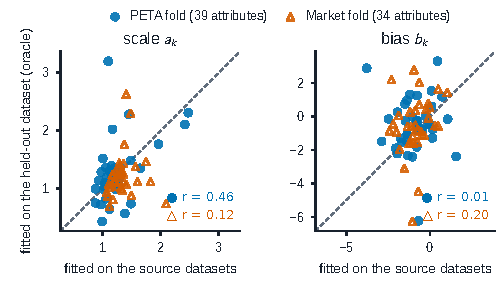
\includegraphics[width=\linewidth]{calib_en.pdf}
\caption{The two parameters of the per-attribute map $\sigma(a_kz+b_k)$, fitted on source data and on the labels of the held-out dataset. Each point is one attribute with enough labels for both fits. The dashed line is $y=x$, and $r$ is the Pearson correlation. Same ensemble as \cref{tab:calib}.}
\label{fig:calib}
\end{figure}

The organizers suggest that models become overconfident or underconfident on new cameras~\cite{upar24}. We test this hypothesis with Platt scaling~\cite{platt} for each attribute, $p=\sigma(a_kz+b_k)$. The map is fitted in two ways. Oracle recalibration fits it on the labels of the held-out dataset itself. It cannot be used at test time, but it shows how many points miscalibration costs. Source recalibration fits it on the validation images of the two source datasets, the only labeled data available in training. This analysis uses the DINOv3 + CLIP ensemble with seed 1 and without WiSE-FT, because only this configuration has saved logits on source data for both folds.

\Cref{tab:calib} shows that miscalibration is real. Oracle recalibration raises mADM by 2.42 points on PETA and 1.60 points on Market-1501. However, source recalibration lowers mADM by about one point on both folds. On the 49 development models, source recalibration lowers mADM for 48 models. The only exception is a model of the PA100k fold, whose training set is much smaller than those of the other folds.

The cause is not that miscalibration appears only on new cameras. On source data, the calibration term is 72\% of that on the held-out dataset in the PETA fold, and it is even larger in the Market-1501 fold. The amount of miscalibration is similar, but its direction for each attribute differs (\cref{fig:calib}). The scale of most attributes is above 1 in both places, so the model is slightly underconfident on both the source data and the held-out dataset. In contrast, the bias of each attribute is almost uncorrelated between the two places. A map fitted on source data therefore shifts the logits of the attributes in directions that do not match the new cameras. A single temperature for all attributes has no per-attribute bias, but it changes mADM by at most 0.4 points in either direction. This result partly confirms the hypothesis of the organizers. Miscalibration costs retrieval points, but the source data do not tell in which direction to correct it. Our system therefore uses the raw probabilities and improves the probabilities themselves with better models.

\subsection{The role of two different encoders}
\label{sec:enc}

\begin{table}[t]
\centering
\small
\setlength{\tabcolsep}{4pt}
\begin{tabular}{@{}lccc@{}}
\toprule
Model & PETA & Market & Mean \\
\midrule
DINOv3 & 66.36 & 73.87 & 70.12 \\
DINOv3, two fine-tuned copies & 66.69 & 74.00 & 70.34 \\
CLIP & 65.81 & 71.72 & 68.76 \\
CLIP + text score & 67.17 & 72.32 & 69.74 \\
CLIP + text score + WiSE-FT & 67.38 & 71.98 & 69.68 \\
\midrule
DINOv3 + CLIP & 68.92 & 74.46 & 71.69 \\
DINOv3 + CLIP (text score) & 69.49 & 74.79 & 72.14 \\
DINOv3 + CLIP (text score, WiSE-FT) & \textbf{69.91} & \textbf{74.90} & \textbf{72.40} \\
\bottomrule
\end{tabular}
\caption{mADM (points) of each model and of the ensembles on the held-out datasets, scored with the likelihood score. Mean is over the two folds. The second row averages the logits of two DINOv3 models, each fine-tuned on its own with the same recipe. An ensemble of two different encoders gains more than an ensemble of two fine-tuned copies of one encoder. The last row is the submitted configuration without the student.}
\label{tab:enc}
\end{table}

Since the probabilities cannot be fixed after training, we improve the probabilities themselves. \Cref{tab:enc} compares each model with the ensembles. Averaging two fine-tuned copies of DINOv3 raises the mean mADM by only 0.22 points over one copy. Adding CLIP to DINOv3 raises it by 1.57 points, although CLIP alone is weaker than DINOv3. The text score and WiSE-FT of the CLIP model add another 0.71 points to the ensemble in the mean, mostly on PETA. The student was trained only for the PETA fold, with 10 epochs instead of the 20 epochs of the submitted student. Adding this student to the ensemble raises mADM on PETA from 69.91 to 70.24 points. We also tried training the two encoders in one network with a joint query head that reads the tokens of both encoders, as in the model we use for Track~1, with the same loss and group CE. This model reaches 69.92 on PETA and 75.04 on Market-1501. Both are below the ensemble with group CE in \cref{tab:gce}, so our Track~2 system keeps the two encoders in separate models.

\subsection{Sensitivity of kNN smoothing}
\label{sec:knn}

\begin{table}[t]
\centering
\small
\setlength{\tabcolsep}{3.5pt}
\begin{tabular}{@{}lcccc@{}}
\toprule
Neighbor feature & $k$, $\alpha$ & PETA & Market & PA100k \\
\midrule
no smoothing (mADM) & & 68.45 & 78.14 & 73.86 \\
\midrule
DINOv3, mean patch token & 3, 0.25 & $-$0.03 & +0.67 & +0.52 \\
DINOv3, mean patch token & 10, 0.25 & +0.56 & +0.86 & +0.67 \\
DINOv3, mean patch token & 20, 0.25 & +0.64 & +0.86 & +0.65 \\
DINOv3, mean patch token & 50, 0.25 & +0.60 & +0.85 & +0.70 \\
DINOv3, mean patch token & 50, 0.2 & +0.70 & +0.69 & +0.66 \\
DINOv3, mean patch token & 20, 0.5 & $-$1.58 & +0.82 & $-$0.29 \\
DINOv3, CLS token & 20, 0.25 & +0.54 & +0.64 & +0.78 \\
CLIP, mean patch token & 20, 0.25 & +0.23 & +1.07 & +0.29 \\
\bottomrule
\end{tabular}
\caption{Change in mADM (points) when the logits are smoothed with \cref{eq:knn}, relative to the first row. The model is the DINOv3 + CLIP ensemble (without text score) of the PETA fold. PETA is the held-out dataset. Market and PA100k are the validation galleries of the two source datasets, whose images were not used in training. The row with $k=50$ and $\alpha=0.2$ is the submitted configuration.}
\label{tab:knn}
\end{table}

\Cref{tab:knn} measures how sensitive kNN smoothing is to $k$, $\alpha$ and the type of feature. It uses an earlier DINOv3 + CLIP ensemble of the PETA fold, with a plain query head for CLIP. Besides the held-out PETA dataset, we evaluate on the validation galleries of Market-1501 and PA100k. These two galleries belong to the source datasets of the fold, but their images were not used in training.

With DINOv3 features, kNN smoothing raises mADM on all three galleries for $k$ from 10 to 50 and $\alpha$ from 0.2 to 0.25. On the held-out PETA dataset, the submitted configuration raises mADM by 0.70 points. When the student is added to the ensemble, the gain on PETA becomes 0.52 points. The values of $k$ and $\alpha$ were chosen on these same galleries, so we report the whole grid. The gain changes little within this range, so it does not come from one carefully chosen setting. With $k=3$, the gain on PETA disappears. With $\alpha=0.5$, the mean of the neighbors has the same weight as the image's own prediction, and mADM on PETA drops by 1.58 points.

The gain comes from the appearance features, not from averaging in general. When the neighbors are found by cosine similarity between the predicted attribute probability vectors, with the same $k=50$ and $\alpha=0.2$, the mADM of the ensemble in \cref{tab:score} changes by $-0.13$ points on PETA and $+0.17$ points on Market-1501. For 44.6\% of the PETA images, the nearest neighbor by DINOv3 features has the same 40 labels as the image. This share is 76.7\% for Market-1501 and 50.6\% for PA100k. \Cref{fig:arch}b shows that the nearest neighbors are often the same person in other frames. DINOv3 features give a larger gain than CLIP features on PETA and PA100k, while CLIP features give a larger gain on Market-1501.

\begin{table}[t]
\centering
\small
\setlength{\tabcolsep}{3.5pt}
\begin{tabular}{@{}lcccc@{}}
\toprule
Held-out & Models & Gains & Median & Range \\
\midrule
PETA & 42 & 42 & +1.08 & {[}+0.11, +1.65{]} \\
Market-1501 & 5 & 5 & +1.12 & {[}+1.00, +1.21{]} \\
\bottomrule
\end{tabular}
\caption{Change in mADM (points) when kNN smoothing ($k=50$, $\alpha=0.2$) with features of the pretrained DINOv3 encoder is applied to the logits of each development model, scored with the likelihood score. Gains is the number of models whose mADM rises. The two models of the PA100k fold have no gallery features and are not counted.}
\label{tab:knngen}
\end{table}

When the neighbor features do not come from the attribute model, kNN smoothing becomes a separate step. It can then be applied to any model without training. \Cref{tab:knngen} applies this step with features of the pretrained DINOv3 encoder to the logits of 47 development models. Every model gains mADM, with a median gain of about one point on both held-out datasets. The gain shrinks as the model gets stronger. On PETA, the Pearson correlation between the starting mADM and the gain is $-0.76$. Models at the weak end gain about 1.6 points, while models at the strong end gain 0.1 to 0.9 points. The submitted ensemble is at the strong end of this range, so its gain in \cref{tab:gce} is smaller.

\subsection{Hidden test set}
\label{sec:test}

\begin{table}[t]
\centering
\small
\setlength{\tabcolsep}{4pt}
\begin{tabular}{@{}p{0.8\linewidth}c@{}}
\toprule
Submission & mADM \\
\midrule
DINOv3 ViT-B/16 student & 63.65 \\
DINOv3 + CLIP + DINOv3 ViT-L/16 student & 67.22 \\
\quad + text score, WiSE-FT, kNN smoothing & 67.83 \\
\quad + group CE for DINOv3 and CLIP & \textbf{68.17} \\
\bottomrule
\end{tabular}
\caption{mADM (points) on the hidden test set of UPAR 2027 Track~2. All submissions use the likelihood score. The 67.83 submission has mAP 39.52, mINP 27.91, Rank-1 40.79, Rank-5 61.45 and Rank-10 69.91.}
\label{tab:test}
\end{table}

\Cref{tab:test} lists the four submissions whose scores were recorded. The first is a single DINOv3 ViT-B/16 student, submitted when the challenge server still ran on the CPU. The next two use the three models in \cref{fig:arch}. The third step changes more than one part, so the contribution of each part cannot be separated, but the direction of the change agrees with \cref{tab:enc,tab:knn}. The last step only replaces the DINOv3 and CLIP models with versions trained with group CE. It raises mADM by 0.34 points, in the same direction as \cref{tab:gce}. This year's leaderboard does not publish a baseline score on the test set, so we cannot compare directly with the baseline.

%=====================================================================
\section{Limitations}
\label{sec:limits}

Our results are measured on the retrieval task of UPAR 2027, with its three datasets and its 40 attributes. We have not tested the likelihood score, group CE or kNN smoothing on other retrieval datasets, and our calibration analysis covers one ensemble and two forms of recalibration. The gain of kNN smoothing depends on how often the same person appears in a gallery, which we could not measure on the hidden test set. Its values of $k$ and $\alpha$ were chosen on the galleries that we report, and most fold results come from a single seed. Attribute-based person retrieval in surveillance video can also be misused to track people without their consent, and this paper reports only technical results.

%=====================================================================
\section{Conclusion}
\label{sec:conclusion}

On unseen cameras, the predictions of fine-tuned foundation encoders should be ranked by the probability of an exact match with the query instead of the L1 distance. Miscalibration costs retrieval points, but it cannot be fixed with data from the source datasets, because the direction of the error for each attribute changes with the domain. Instead, two ways of improving the probabilities themselves carry over to a new dataset. Group CE teaches the model that exactly one value of each mutually exclusive group is present, and the appearance features of the encoder let the gallery smooth its own predictions. A next step is to test kNN smoothing on galleries with few repeated images of the same person.

{\small
\bibliographystyle{ieeenat_fullname}
\bibliography{refs}
}

\end{document}
